% !Mode:: "TeX:UTF-8" 

\BiChapter{基于条件编码长短期记忆社交媒体文本立场分析}{Methods of inserting figures}

\BiSection{引言}{Figures inserting standard from graduate school}
当前社交媒体文本立场分析的研究中,研究人员的研究方向主要集中在如何提取社交媒体文本有效的分类特征。忽略了文本立场分析一种重要的出发点是文本基于某个特定的目标,若原文本脱离了特定目标,文本立场分析与情感分析将无差别。基于这个出发点,本章提出了基于条件编码长短期记忆神经网络的模型,通过以条件编码的形式引入文本的主题目标信息,使立场分析的效果得到显著的提升。本章研究基于条件编码长短期记忆的社交媒体文本立场分析方法,通过以不同形式给模型接入文本立场的主题目标信息,表明了接入目标信息对文本立场分析有明显提升效果。通过在SemEval2016英文立场分析数据集和NLPCC2016中文立场分析数据集的实验,论证上述结论。

本章的各节结构如下:3.2节介绍条件编码长短期记忆神经网络模型;3.3节介绍基于条件编码长短期记忆在文本立场分析;3.4 节为本章实验和结果分析;最后一节为本章小结。

\BiSection{条件编码长短期记忆神经网络模型}{Captions and descriptions of figures}
循环神经网络(Recurrent Neural Networks, RNN)已经在众多自然语言处理任务上取得了巨大成功。不同于传统的前向反馈神经网络的同层节点无连接层于层之间节点有连接,循环神经网络引入了定向循环,可以处理序列数据。RNN中最大的缺陷是后面时间的节点对于前面节点的感知力下降,当网络深时训练效果下降。LSTM可以解决这一问题,目前LSTM是RNN中使用最广泛最成功的模型。Rocktaschel[???]在2016年在句子之间的文本蕴含识别(Recognizing textual entailment,RTE)的研究中提出了条件编码的思想,其论证了在文本含义识别任务上,条件编码比单独编码更能抽取两个句子之间的信息。结合文本立场分析的也有文本和目标需要同时考虑特点,把借鉴条件编码的思想来解决文本立场分析的任务。
\BiSubsection{基于GloVe的词嵌入模型}{}
词的表示是自然语言处理中一个基础且十分重要的任务,大量的研究人员投入到词表示的研究中。早期的有词的表示方式为one hot encoding。每个词独占一个维度,每个词向量有一个维度是1,其他维度为0,词向量的维度是所有单词的的长度。One hot编码的特点是假设所有的单词互相独立,这是一个很强的假设,显然在有些任务中并不合适,如词语相似度方面,dog和cat的相似度应当比dog和not高,但是在one hot编码中他们相似性一样。one-hot编码词表示有一些缺点,如容易受位数灾难的困扰,且不能很好地刻画词与词之间的相似性。词嵌入表示模型能很好的改善one-hot编码的缺点,词的嵌入模型用稠密且固定长度的向量表示每一个词,而且相似的词具有相似的词向量表示。基于这点Mikolov[??]2013提出了Word2Vec模型,解决了词向量训练速度慢,效率低的缺点。其利用了CBOW(Continuous Bag-of-words Model)和Skip-Gram的两种语言模型。其中CBOW的思想是利用词语的上下文词的信息来预测该单词。而Skip-Gram则采取一种和CBOW相反的策略,用中间的词的消息来预测上下文的词。GloVe(Global Vectors for Word Representation)是斯坦福大学发表的一种词嵌入模型,GloVe尝试借鉴NNLM和word2vec的优势来弥补旧方法的劣势,取得了不错的效果。该文发表于Word2Vec之后,其方法内核比较朴实和简单,官方实验中,GloVe是略胜Word2Vec一筹。

\begin{figure}[htbp]
	\centering
	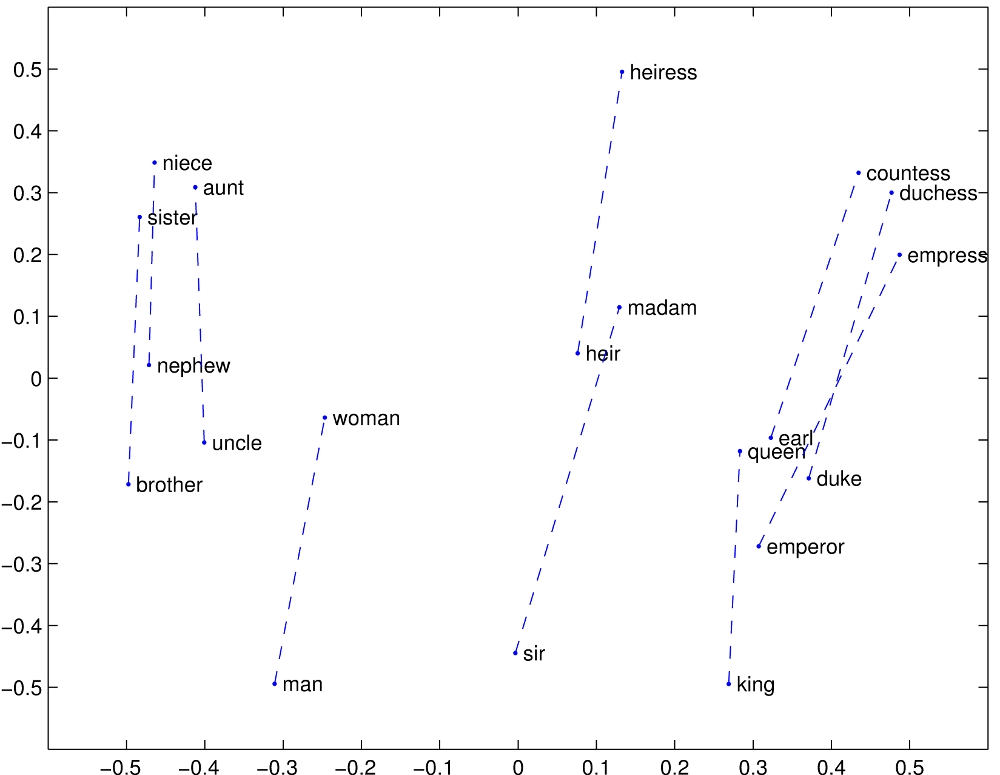
\includegraphics[width = 0.6\textwidth]{glove.jpg}
	\caption[rnn_vanish]{GloVe可视化词向量}
\end{figure}

GloVe结合了基于矩阵分解的词嵌入表示和基于语言模型(例如Word2Vec)的词嵌入表示。基于矩阵分解具有训练快,容易实现的优点,但是生成词向量语义信息十分有限。基于语言模型的词嵌入表示则具有更多语言学层次的支持,在更多自然语言处理任务上表现更好,但是模型关注的上下文特征较少,忽略了全局的信息。GloVe发明的初衷,就是想结合两者的长处,建立一个充分利用统计量的更好训练的适用程度更广的词嵌入模型。具体模型建立公式如下

$$ F(w_i,w_j,w^c_k) = \cfrac{P_{ij}}{P_{jk}} $$
其中,取$word_i$的出现次数为$X_i$, 定义$P_{ij}=P(j|i)=\cfrac{X_{ij}}{X_{i}}$表示在$X_i$的上下文下$word_i$的出现几率, $F$则是某一种能够实现我们需求的变换。$w_i,w_j$是实数空间下的$word_i,,word_j$的词向量,$w^c_k$也是实数空间下的$word_k$的上下文词向量,其作用类似Word2Vec中的上下文向量。为了精简计算引入词向量的线性加减和点乘计算
$$ F((w_i-w_j)^Tw^c_k) = \cfrac{F(w^T_iw^c_k)}{{F(w^T_jw^c_k)}} $$
GloVe每个词涉及到两个词向量,一个词语本身的向量$w_i$,一个词的context向量$w^c_i$。最初这样设计,将词向量和上下文的向量分开,不用一套,是为了在更新参数的时候能够简单地套用SGD。实验证明两个向量加起来最后起到的效果最好。后面英文的词向量用的是GloVe模型在大量的Twitter文本上训练的100维度的词向量,中文微博词向量是200维度的词向量。

\BiSubsection{长短期记忆神经网络模型}{Layouts of illustrations}
由于文本序列的通常具有较长的长度,导致神经网络的层数较多,而传统的递归神经网络解决序列问题经常会出现梯度消失的问题(vanishing gradient problem)与梯度爆炸问题(gradient exploding problem)。梯度消失问题和梯度爆炸问题一般随着网络层数的增加会变得越来越明显。出现的原因在于对神经网络参数进行链式求导的过程中,输出对于前面递归神经参数的倒数随着累乘激活函数的导数而接近于0,以下图的反向传播为例(假设每一层只有一个神经元且对于每一层$y_i=\sigma(z_i)=\sigma(w_ix_i+b_i)$,其中$\sigma$为sigmoid函数)

\begin{figure}[htbp]
	\centering
	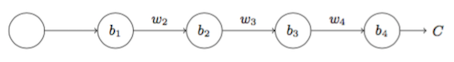
\includegraphics[width = 0.7\textwidth]{rnn_gradient_vanish.png}
	\caption[rnn_vanish]{RNN梯度消失}
\end{figure}

可以推导出

\begin{equation}\label{nodelimiter}
\frac{\partial C}{\partial b_1} = \frac{\partial C}{\partial y_4}\frac{\partial y_4}{\partial z_4}\frac{\partial z_4}{\partial x_4}\frac{\partial x_4}{\partial z_3}\frac{\partial z_3}{\partial x_3}\frac{\partial x_3}{\partial z_2}\frac{\partial z_2}{\partial x_2}\frac{\partial x_2}{\partial z_1}\frac{\partial z_1}{\partial b_1}
\end{equation}
\begin{equation}\label{delimiter}
=\frac{\partial C}{\partial y_4}\ \sigma ^\prime(z_4)w_4\sigma ^\prime(z_3)w_3\sigma ^\prime(z_2)w_2\sigma ^\prime(z_1)
\end{equation}

一般的非线性激活函数的导数都小于1(例如sigmoid的导数最大值为$\frac{1}{4}$),因此对于上面的链式求导,层数越多,求导结果$\frac{\partial C}{\partial b_1}$越小,因而导致梯度消失的情况出现。
长短期记忆(Long Short-Term Memory, LSTM)是一种缓解上述问题的间递归神经网络的变种,Hochreiter在1997年首次提出了LSTM结构,2000年Gers等人改进LSTM模型。

\begin{figure}[htbp]
	\centering
	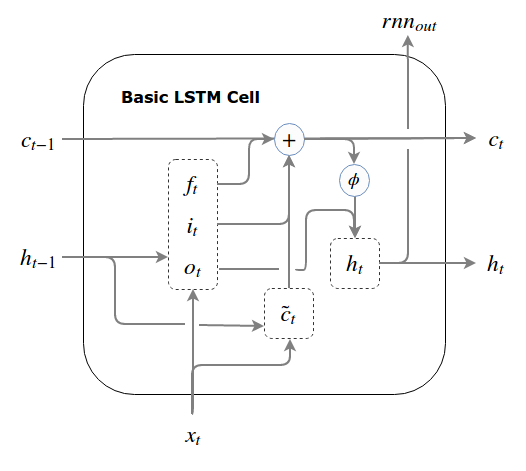
\includegraphics[width = 0.6\textwidth]{lstm_unit.png}
	\caption[rnn_vanish]{LSTM单元结构}
\end{figure}

LSTM模型提出了记忆存储格(memory cell)的结构,内部包含了遗忘门(forget gate)、输入门(input gate) 和输出门(output gata) 。各种门的作用在于调节记忆体在外部输入的情况下应该采取怎么的存储测量,具体门状态和记忆体内部参数的更新公式如下。

\begin{equation}\label{lstm_f}i_t=\sigma_g(W^ix_t+U_ih_{t-1}+b^i)\end{equation}
\begin{equation}\label{lstm_f}f_t=\sigma_g(W^fx_t+U_fh_{t-1}+b^f)\end{equation}
\begin{equation}\label{lstm_f}o_t=\sigma_g(W^ox_t+U_oh_{t-1}+b^o)\end{equation}
\begin{equation}\label{lstm_f}c_t=f_t \odot c_{t-1}+i_t\odot \sigma_c(W_cx_t+U_ch_{t-1}+b_c)\end{equation}
\begin{equation}\label{lstm_f}h_t=o_t \odot \sigma_h(c_t)\end{equation}

其中$\sigma_g$为sigmoid的激活函数,$\sigma_c, \sigma_h$为thah的激活函数,$x_t$为输入向量,$h_t$为输出向量, $c_t$为记忆向量,$W,U,b$是矩阵参数和向量参数。各个门的值是保持在0-1之间的向量。其中遗忘门向量$f_t$表示上一时刻的记忆体信息需要遗忘多少, 输入门向量$i_t$表示有多少当前时刻输入信息需要加入到记忆体中,输出门向量$o_t$表示记忆体输出多少信息。

研究人员已经证明,LSTM是解决长序依赖问题的有效技术,并且这种技术的普适性非常高,导致带来的可能性变化非常多。各研究者根据LSTM纷纷提出了自己的变量版本,这就让LSTM可以处理千变万化的垂直问题。

\BiSubsection{条件编码长短期记忆神经网络模型}{}
Rocktaschel[]等在句子之间的文本蕴含识别的研究中提出了条件编码长短期记忆神经网络模型,文本蕴含定义为一对文本之间的有向推理关系,其中蕴含前件记作T(Text),蕴含后件记作H(Hypothesis)。如果人们依据自己的常识认为H的语义能够由T的语义推理得出的话,那么称T蕴含H,记作T → H, 作者提出的模型的结构是首先有一个LSTM模型编码Text消息,另一个不同参数的LSTM模型编码Hypothesis。作者不是简单把两个特征向量拼接在一起,而是做了如下转换。把第一个编码Text信息的LSTM模型的记忆状态(Cell)保留下来,作为第二个编码Hypothesis的LSTM模型记忆状态(Cell)的初始值,此模型建立的了Text消息作为条件下的对Hypothesis的编码表示。

\begin{figure}[htbp]
	\centering
	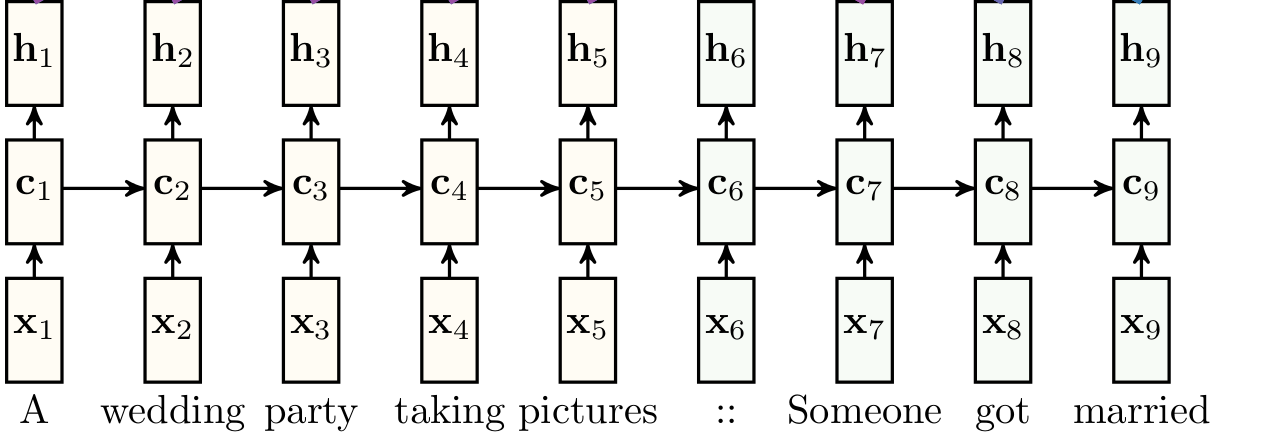
\includegraphics[width = 0.8\textwidth]{conditional_encoding.png}
	\caption[rnn_vanish]{条件编码长短期记忆}
\end{figure}

如上图图表示所示“A wedding party taking pictures”作为我们的Text文本,“Someone got married”作为我们的Hypothesis,其中$c_5$作为前一个LSTM的记忆体状态被当做编码Hypothesis的初始记忆状态。两个LSTM具体的状态转移公式如下:
\begin{equation}\label{lstm_f}[h_1~c_1] = LSTM^{Text}(x_1,h_0,c_0)\end{equation}
$$...$$
\begin{equation}\label{lstm_f}[h_T~c_T] = LSTM^{Text}(x_1,h_{T-1},c_{T-1})\end{equation}
\begin{equation}\label{lstm_f}[h_{T+1}~c_{T+1}] = LSTM^{Hypothesis}(x_1,h_0,c_T)\end{equation}
$$...$$
\begin{equation}\label{lstm_f}[h_{N}~c_{N}] = LSTM^{Hypothesis}(x_1,h_{N-1},c_{N-1})\end{equation}
\begin{equation}\label{lstm_f}c=tanh(Wh_N)\end{equation}
其中$(x_1...x_T)$为Text的序列消息,$(x_{T+1}...x_N)$为Hypothesis的序列信息。$h_0,c_0$为LSTM的初始化向量。

实验证明在文本蕴含任务上,条件LSTM模型比单独编码高3.3\%(从77.6\%提升到80.9\%)的性能。这种条件编码能使Text的信息更好的流向对Hypothesis编码的LSTM模型,有了第一个LSTM模型传来的记忆状态,第二个LSTM模型能更好的编码Hypothesis的消息。

\BiSection{基于条件编码长短期记忆的文本立场分析}{}

通过Rocktaschel在文本蕴含的任务的实验可知,在处理两个文本序列的编码任务上,条件编码长短期记忆神经网络比单独独立编码两个文本序列有更好的建模能力。在文本立场分析的任务上,有文本的信息和目标主题两个文本序列信息,我们可以借鉴条件编码长短期记忆神经网络在文本蕴含建模的方式,把文本信息和目标主题信息更好结合起来。在实验部分设计了多种文本序列信息的结合方式,通过实验证明了以目标主题文本作为条件编码文本信息的模型对文本立场分析有更好的效果。

本文后期实验将在NLPCC2016中文微博立场分析数据集和SemEval2016英文Twitter立场分析数据集,为较清晰阐述条件编码长短期记忆模型,以下简短的介绍下两个数据集的样例,具体的有关数据集的信息将会在下面实验部分做详细介绍。

例1:目标主题文本:"深圳禁摩限电" 微博文本:"支持深圳交警。电单车继续治理" 立场分析类标:“Favor”(持支持立场)

目标的文本主题有关“深圳禁摩限电”的主题的,而从微博文本“支持深圳交警。电单车继续治理”中,我们可以知道微博的作者首先是赞同了深圳交警的行为,然后叙述了电单车需要得到继续的整治,从两个方法肯定了"深圳禁摩限电"这个主题目标的,因此给出的类标是“Favor”也就是持支持目标主题的立场。

例1:目标主题文本:"Hillary Clinton" Twitter文本:"Hopefully Hillary Clinton gets cancer and dies before she gets the opportunity to embarrass our country any further“,立场分析类标“Against”(持反对立场)

译文:"真希望希拉里克林顿得癌症然后死去,这样她就不再会有机会再让我们国家蒙羞了。"

目标的文本主题有关“希拉里克林顿”的主题的,这个Twitter文本是有关2016年美国大选,显然Twitter作者一直咒骂希拉里克林顿,希望她得癌症,不让她侮辱国家,可以看出作者有强烈反对主题目标“希拉里克林顿”,因此给出的类标是“Against”,也就是持反对目标主题的立场。

从上述的两个简单的样例可知,立本立场是有两个输入的,一个是立场主题例如“深圳禁摩限电”和“Hillary Clinton”。另外一个是立场下的文本“支持深圳交警。电单车继续治理”和”Hopefully Hillary Clinton gets cancer and dies before she gets the opportunity to embarrass our country any further“。在这通过中文微博阐述条件编码长短期记忆模型的建立。首先经过一些数据预处理和分词把主题目标”深圳禁摩限电“和”支持深圳交警。电单车继续治理”转变成”深圳 禁摩 限电“和”支持 深圳 交警 电单车 继续 治理“。

在文本立场分析的任务, 一般目标主题包含的信息较少,而文本包含了大部分的信息。例如上面两个例子所举例的,目标主题文本分别为”Hillary Clinton“和”深圳禁摩限电“,而Twitter和微博文本包含的消息较多,结合立场分析文本的特点,改善了原有的条件编码长短期记忆的网络结构,后续实验论证在多种条件编码长短期记忆的改进方案中,下面所示的网络结构具有更好的实验效果,后续在实验分析其可能的原因。

\begin{figure}[htbp]
	\centering
	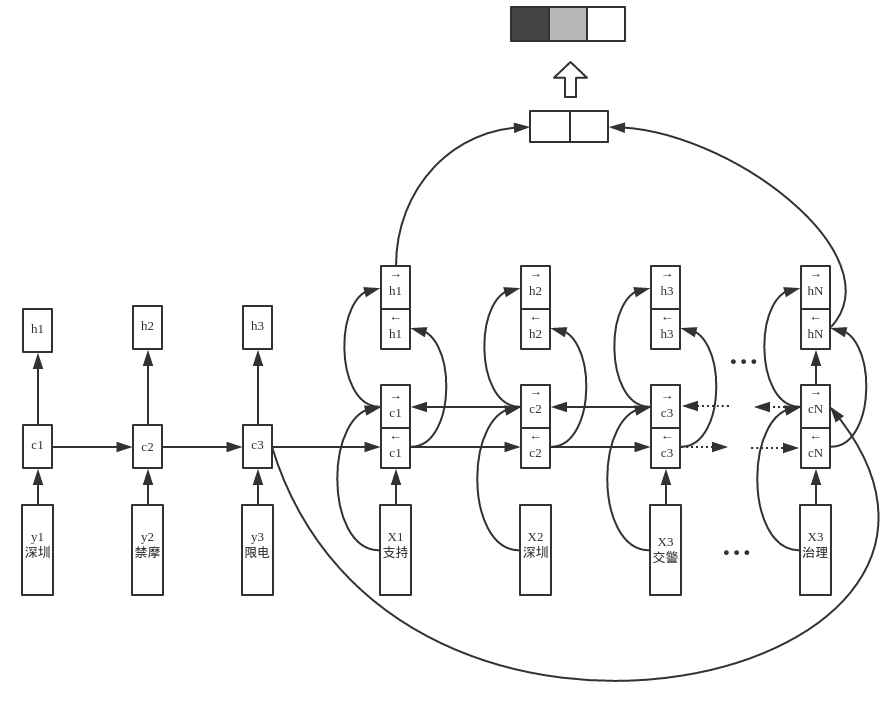
\includegraphics[width = 0.85\textwidth]{conditional_encode_lstm3.png}
	\caption[rnn_vanish]{条件编码长短期记忆}
\end{figure}

模型的具体公式如下

\begin{equation}\label{lstm_f}[h_1~c_1] = LSTM^{target}(t_1,h_0,c_0)\end{equation}
$$...$$
\begin{equation}\label{lstm_f}[h_M~c_M] = LSTM^{target}(t_1,h_{M-1},c_{M-1})\end{equation}

\begin{equation}\label{lstm_f}[h^{forward}_{1}~c^{forward}_{1}] = LSTM^{forward}(x_1,h_0,c_T)\end{equation}
$$...$$
\begin{equation}\label{lstm_f}[h^{forward}_{N}~c^{forward}_{N}] = LSTM^{forward}(x_n,h^{forward}_{N-1},c^{forward}_{N-1})\end{equation}

\begin{equation}\label{lstm_f}[h^{backward}_{N}~c^{backward}_{N}] = LSTM^{backward}(x_n,h_0,c_T)\end{equation}
$$...$$
\begin{equation}\label{lstm_f}[h^{backward}_{1}~c^{backward}_{1}] = LSTM^{backward}(x_1,h^{backward}_{2},c^{backward}_{2})\end{equation}

\begin{equation}\label{lstm_f}c_i=Softmax(W[h^{forward}_n~h^{backward}_1])\end{equation}

其中$M$为主题目标的文本长度,$N$为微博或Twiiter的文本长度。$LSTM$单向编码主题目标,$LSTM^{forward}$为前向编码文本信息,$LSTM^{backward}$为后向编码文本信息,$h_0$为LSTM的初始化向量,$C_T$为$LSTM$主题目标编码的最后一个Cell状态,$h^{backward}_{1},h^{forward}_{N}$分别为前向和后向编码的最后一个隐藏状态。

本节以“深圳禁摩限电”为话题目标,微博文本“支持深圳交警。电单车继续治理”为例,按本节模型的5个层次,描述基于条件编码长短期记忆的立场分析的过程。

(1)输入层

先将话题目标和微博文本经过预处理操作,然后通过分词工具把话题目标和微博文本进行划分,对于同一个话题目标,微博文本分词后句子长度有可能不一致,为了方便后续神经网络框架中的批量的并行计算,通过统计选择30为固定长度,长度超过固定长度进行截断操作,不够的进行补齐词表中规定<PAD>关键词。如例微博文本最后转换成”支持 深圳 交警。电单车 继续 治理 <PAD> ... <PAD>“

(2)词向量嵌入层

词向量的嵌入层,此层的功能是对输入的每一次词检索其词向量(lookup操作),后续实验词向量的预训练由GloVe模型在大量无监督语料上训练可得,预训练的词向量维度为100,且把词向量设置为可训练,随神经网络模型的训练动态调整权重。

(3)主题目标编码层

通过一个单向的长短期记忆(LSTM)模型模型编码主题目标,把分词后的主题目标“深圳 禁摩 限电”通过lookup操作取出相应的词向量,经过一个隐藏层为64的单向LSTM模型,且保留最后的记忆体的状态,如上图所示,保留XXX的单元的信息,给下一层文本编码做输入。

(4)文本编码层

由于文本包含大部分信息,所以采用了双向的LSTM模型而不是Rocktaschel提出的单向的LSTM模型编码文本信息。如上图所示,文本编码的双向LSTM模型的初始Cell状态是由上一层的目标主题编码的最后的Cell状态填充,表示主题目标的消息流入到当前的双向LSTM模型中参与对文本的编码操作。每一个方向LSTM的最后的隐状态h作为对整个文本的最终编码表示。

(5)全连接层


全连接层接受来自文本编码层每个方向最后的隐状态,拼接两个隐状态信息作为最后的特征向量。全连接层的输出个数为3,表示每个立场的预测概率。通过softmax激活函数归一化三个立场的概率,在预测阶段我们选取概率最大的立场当做预测的类标。

\BiSection{实验设置及结果分析}{hello}

本节主要介绍条件编码长短期记忆神经网络模在2016NLPCC微博中文语料库和2016SemEval英文Twitter数据集中的实验结果及分析。并从实验的角度论证条件编码长短期记忆在立场分析问题上的有效性。本节包含两部分: 3.4.1 小节介绍中英文两个数据集中训练和测试文本的分布 、实验评价方式以及对比方法;3.4.2 小结介绍模型训练阶段的性能调优,以及本章实验与其他方法的比较。

\BiSubsection{实验设置}{}

(1)数据集简介

为验证条件编码长短期记忆神经网络在立场分析任务上算法的性能表现,本节采用2016 NLPCC中文微博语料和2016 SemEval英文的Twitter语料两个数据集验证算法的效果。以下分别介绍两数据集的分布。

中文数据集来自NLPCC2016 立场分析测评任务[55] ,数据集的5个话题目标分别为 iPhone SE、春节放鞭炮、俄罗斯在叙利亚的反恐行动、开放二胎政策和深圳禁摩限电。所有语料都来自于新浪微博,每个微博文本的立场属于“支持”、“反对”和“其他”三者之一。NLPCC 2016中文微博数据集的训练集、测试集按照75\%与25\%的比例划分,如表~\ref{chinesedata}~所示详细介绍每个话题目标下数据的分布。
\begin{table}[htbp]
	\caption[table123]{训练集、测试集话题数量及立场分布比例(中文数据集)}
	\label{chinesedata}
	\vspace{0.5em}\centering\wuhao
	\begin{tabular}{cccccccccc}
		\toprule[1.5pt]
		\multirow{2}{*}{预置话题分类}& \multicolumn{4}{c}{训练集数量和立场比例(\%)} 
		& \multicolumn{4}{c}{测试集数量和立场比例(\%)}  &\multirow{2}{*}{文本数量}\\
		\cline{2-9}
		\quad&数量& 支持&反对&其他&数量& 支持&反对&其他 \\
		\midrule[1pt]
		iPhone SE&600&40.8&34.8&24.3&200&37.5&52.0&10.5&800\\
		春节放鞭炮&600&41.7&41.7&16.7&200&44.0&47.0&9.0&800\\
		俄在叙反恐行动&600&41.7&41.7&16.7&200&47.0&43.0&10.0&800\\
		开放二胎政策&600&43.3&33.3&23.3&200&49.5&47.5&3.0&800\\
		深圳禁摩限电&600&26.7&50.0&23.3&200&31.5&55.0&13.5&800\\
		总计&3000&38.8&40.3&20.9&1000&41.9&48.9&9.2&4000\\
		\bottomrule[1.5pt]
	\end{tabular}
\end{table}

英文数据集来自SemEval2016 Task6 stance detection[55] ,数据集的5个话题目标分别为 Atheism(无神论)、Climate Change is a Real Concern(气候变化真实性)、Feminist Movement(女权运动)、 Hillary Clinton (希拉里克林顿)和
Legalization of Abortion(堕胎合法化)。所有语料都来自于英文Twitter文本,每个Twitter文本的立场属于“支持”、“反对”和“其他”三者之一。不同于上述中文语料的分布,每个话题目标英文Twitter语料的数量参差不齐,但总体上训练集和测试集按70\%与30\%的比例划分,如表~\ref{englishdata}~所示详细介绍每个话题目标下数据的分布。


\begin{table}[htbp]
	\caption[table123]{训练集、测试集话题数量及立场分布比例(英文数据集)}
	\label{englishdata}
	\vspace{0.5em}\centering\wuhao
	\begin{tabular}{cccccccccc}
		\toprule[1.5pt]
		\multirow{2}{*}{预置话题分类}& \multicolumn{4}{c}{训练集数量和立场比例(\%)} 
		& \multicolumn{4}{c}{测试集数量和立场比例(\%)}  &\multirow{2}{*}{文本数量}\\
		\cline{2-9}
		\quad&数量& 支持&反对&其他&数量& 支持&反对&其他 \\
		\midrule[1pt]
		Atheism&513&17.9&59.3&22.8&220&14.5&72.7&12.7&733\\
		Climate Change&395&53.7&3.8&42.5&169&72.8&6.5&20.7&564\\
		Feminist Movement&664&31.6&49.4&19.0&285&20.4&64.2&15.4&949\\
		Hillary Cliton&689&17.1&57.0&25.8&295&15.3&58.3&26.4&984\\
		Legal of Abortion&653&18.5&54.4&27.1&280&16.4&67.5&16.1&933\\
		总计&2914&25.8&47.9&26.3&1249&24.3&57.3&18.4&4163\\
		\bottomrule[1.5pt]
	\end{tabular}
\end{table}

为了和已有方法进行性能比较,本文在两数据集上都按照分别测评的比例划分出训练集和测试集。其中训练集负责模型的训练和调优, 测试集则进行最后模型的性能的评估。中英文数据集均包含5个不同的话题目标, 每个话题目标包含若干的话题文本,由于每个主题目标关注的内容不同且具有各自独特的语言特点。为了使模型更好的拟合每一种话题的特性,本文首先按照中英文不同语料集合划分成两个大任务,然后根据每个语料库在细分成5个不同子任务,分别建立不同的条件编码长短期记忆模型。各子模型预测结束后, 统计各个子任务上的性能并汇总预测结果进行最后统一指标的计算。

(2)评价指标

中英文数据集上的社交媒体文本的立场结果有“支持”,“反对”,“其他”,可以把任务当成一个三分类任务,但是由于三个类在不同的数据集下的不同主题目标的分布有可能很不平均,如果只单独用正确率(Accuracy)作为评测指标则缺失了评价指标的客观性。本文c采取了两个评测任务都使用的”支持“和”反对“的F1指标的微平均(micro-average)作为最后模型的评测指标,但是为了更清晰的评价每个主题目标的性能,每个目标主题也会单独计算微平均评测指标。为了清晰地解释指标的含义,列举以下公式说明

首先定义准确率(Precision, P)、召回率(Recall, R),如公式~\ref{precision}~和公式~\ref{recall}~所示。
\begin{equation}\label{precision}P=\frac{TP}{TP+FP}\end{equation}
\begin{equation}\label{recall}F=\frac{TP}{TP+FN}\end{equation}

TP:正样例预测为正样例的个数

FP:负样例预测为正样例的个数

FN:正样例预测为负样例的个数。

精确率计算的是所有"正确被检索的样例(TP)"占所有"实际被检索到的(TP+FP)样例的比例。召回率计算的是所有"正确被检索的运力(TP)"占所有"应该检索到的样例(TP+FN)"的比例。如果要同时考虑精确率和召回率,则需要采样两者的调和平均值,也称为F1值,其定义如公式~\ref{f1score}~所示
\begin{equation}\label{f1score}F1=\frac{2PR}{P+R}=\frac{2TP}{2TP+FP+FN}\end{equation}

有关”支持“立场F1值的计算,“支持”类标作为正样本,“反对”后“其他”作为负样本。因此其计算公式如下所示

\begin{equation}\label{f1favor}F1_{favor}=\frac{2P_{favor}R_{favor}}{P_{favor}+R_{favor}}\end{equation}

同样的”反对“立场F1值的计算,“反对”类标作为正样本,“支持”后“其他”作为负样本。因此其计算公式如下所示

\begin{equation}\label{f1against}F1_{against}=\frac{2P_{against}R_{against}}{P_{against}+R_{against}}\end{equation}

立场分析总的平均指标F1的微平均(Micro-average)的计算公式如下
\begin{equation}\label{f1average}F1_{average}=\frac{F1_{favor}+F1_{against}}{2}\end{equation}

本文实验的社交媒体立场分析数据都来自于新浪微博或者Twitter,此类网络语言文本具有文本形式极度不规范,口语化严重。Twitter与微博是由网络用户即兴创作的短文本,用户在用词、语法等方面随意性较大,文本形式与新闻、维基百科等语料具有很大的差异。由于Twitter和微博一般有对单条文本长度做出文本长度的限制,因此这些网络文本中常含有缩写、俗语、流行词汇等元素,同样也存在语法成分缺失的问题。除此之外,文本中大量存在的网页链接、“@某用户”和“\#某话题”等功能标记。

由于社交媒体文本根据上述特点,分别对中英文语句进行预处理操作。删除语料中其中的大量URL信息,由于“\#某话题”等话题标签对立场分析有很重要的影响,因此把话题标签消息保留了下来,对于英文所有词语全转换成小写拼写,分词工具采用了CMU专门为Twitter开发的Twitter NLP tool里面的分词模型[XXX], 中文的分词工具采用较为稳定的结巴分词工具。对于网络社交文本分词后可转换成一些词语的序列信息,对于在训练集中出现次数小于2词的词语归为低频词,为了减少模型的参数,加大模型的泛化能力,把所以的低频词转换成一个统一的词汇用“UNKNOW”标识。同时为了兼容现在主流的基于批量更新的深度学习框架,对文本的长度进行固定操作。英文的文本固定为30个词的长度,中文微博文本固定为50的词长度。

英文语料的词向量训练通过GloVe算法在20亿Twitter文本语料训练而成,其中包含了120万个词,词向量维度为200。中文微博语料是通过Word2Vec算法在大量微博语料中训练所得,其中包含了17万个词,词向量的维度也为200。

本文建立了针对5个不同话题目标的子模型, 使用相同的条件编码长短期记忆模型参数。取出训练集合的10\%作为验证集参与模型的选择。通过实验发现,当对主题目标和文本编码LSTM模型的隐藏层单元设置为64,embedding层的dropout的概率设置为0.2,当对主题目标和文本编码LSTM模型内部记忆的dropout概率设置为0.3,每次以32个样本作为mini-batch参加参数更新,选取0.001的学习率的Adam优化方法。

\begin{table}[htbp]
	\caption[param]{基于条件双向编码长短期记忆的立场分析实验超参数集}
	\label{param}
	\vspace{0.5em}\centering\wuhao
	\begin{tabular}{ccc}
		\toprule[1.5pt]
		序号& 超参数名称 &数值\\
		\midrule[1pt]
		1 &LSTM隐藏层单元& 64\\
		2 &Embedding层dropout& 0.2\\
		3 &LSTM内部drought& 0.3\\
		4 &批处理大小& 32\\
		5 &L2 正则化参数 &1e-6\\
		6 &全量迭代次数& 50\\
		7 &梯度优化方法& Adam\\
		8 &学习率& 0.001\\
		\bottomrule[1.5pt]
	\end{tabular}
\end{table}

\BiSubsection{实验结果及分析}{}
通过网格搜索调节不同参数,使得基于条件双向编码长短期记忆模型在各个数据集上取得最优的效果。调优过程中,在模型的词向量抽取层、LSTM内部记忆单元层、和最后的特征向量层加入适当的dropout可以使得模型更加的稳定,Dropout一定层度上减少了模型过拟合的趋势,增加了模型的泛化能力,通过调节最优参数,模型在SemEval2016数据集上的表现表~\ref{conditional_semeval}~所示。
\begin{table}[htbp]
	\caption[table123]{条件双向编码长短期记忆模型在各个话题试验性能(SemEval数据集)}
	\label{conditional_semeval}
	\vspace{0.5em}\centering\wuhao
	\begin{tabular}{cccccccc}
		\toprule[1.5pt]
		主题目标& $P_{favor}$&$R_{favor}$&$F_{favor}$&$P_{against}$&$R_{against}$&$F_{against}$&$F_{average}$ \\
		\midrule[1pt]
		Atheism&0.3824&0.4063&0.3939&0.8323&0.8375&0.8349&0.6144\\
		Climate Change&0.7389&0.9431&0.8286&0.0000&0.0000&0.0000&0.4143\\
		Feminist Movement&0.3924&0.5345&0.4526&0.7205&0.6339&0.6744&0.5635\\
		Hillary Clinton&0.6316&0.2667&0.3750&0.6638&0.8837&0.7581&0.5666\\
		Legal. of Abortion&0.4630&0.5435&0.5000&0.7770&0.6085&0.6825&0.5912\\
		合并统计&0.5743&0.6480&0.6112&0.7396&0.7231&0.7314&0.6713\\
		\bottomrule[1.5pt]
	\end{tabular}
\end{table}

如表~\ref{conditional_semeval}~所示,以下分析模型的结果。条件双向编码LSTM模型在所有类标的micro-F1值的指标为0.6713,其总结所有主题目标“支持”立场的F1值为0.5789,而“反对”立场的总体F1值有0.7418。从这个数据可以看出来模型对反对立场有更好的性能,模型会有这样的偏置的原因是由于原英文数据的分布有关,原英文数据集的分布如表~\ref{englishdata}~所示,训练集0.47的样本是持”反对“立场,测试集合也有0.57的持反对立场。而“支持”立场分别只占了0.25和0.24。由于有更多的“反对”样本,条件双向编码LSTM模型能更好的识别”反对“立场中的分类模型,并且模型在不平均数据集上会对高频的类有先天的偏置。这两点导致了模型在“反对”立场上的性能比“支持”有更好的性能。单独分析具体话题目标,“Climate Change is a Real Concern”主题目标的F1值只有0.41,远低于其他主题目标的指标。从原数据分析发现,“Climate Change is a Real Concern”主题目标下”反对“立场只占原数据集的0.03,”支持“的占有率为0.53,”支持“的样本是“反对”的10多倍了。而从模型最后对于“反对”测试集准确率为0,召回率也为0。可以看出最后模型都未预测任何一个样本为“反对”立场,这导致了模型在“Climate Change is a Real Concern”的准确率和召回率都为0,其次训练集和测试集在“Climate Change is a Real Concern”上的分布也有较大的差距,支持立场在训练和测试集合中有将近20\%的差距,这样一点程度上影响模型在此主题目标下的性能,最终影响了整体的模型性能。

如表~\ref{conditional_semeval}~所示,整体模型的Micro-F1值为0.6713。远高于性能好的子主题目标"Atheism"上的F1值0.6114。其中的原因有可能是各个主题目标的“反对”和“支持”分布较不均匀,例如“Climate Change is a Real Concern”中“支持”立场占了0.53,而“Hillary Clinton”中”反对“立场占据了0.57。相对来说单个主题目标中“支持”与”反对“的分布很均衡,但整体综合5个主题目标后,“支持”与”反对“却变得相互平衡了。因此导致"支持”和“反对”立场都拥有了较好了F1指标,进一步micro-F1的指标也会优于各个主题目标的F1指标。

在NLPCC2016数据集上,采取对编码主题目标和微博文本的LSTM隐藏单元为设为100,其他超参数和SemEval英文数据一样。在此数据集上综合5个主题目标,“支持”立场的F1值为0.665,“反对”立场的F1值为0.707,总体的Micro-F1值为0.686。

在NLPCC2016数据集上,每个主题目标的性能如表~\ref{chinese_condition}~所示,“俄罗斯在叙利亚的反恐行动”的平均F1指标只有0.583,其他指标都上了0.6,而“春节放鞭炮”主题目标的F1平均值到达了0.745,说明模型在此数据集的性能相对较好。原始数据的分布也造成此现象的根本原因。中文文本的训练数据和测试数据如表~\ref{chinesedata}~所示,除了“深圳禁摩限电”主题目标外,其他4个主题目标的”支持“立场大概占据0.4左右的比例,而“反对”立场则占据0.35左右的。而且测试集合和训练集合的分布相似度极高,因此模型在中文数据集相对的性能就比较高。
\begin{table}[htbp]
	\caption[table123]{基于子话题分别训练的条件双向编码长短期记忆模型试验性能(SemEval数据集)}
	\label{chinese_condition}
	\vspace{0.5em}\centering\wuhao
	\begin{tabular}{cccccccc}
		\toprule[1.5pt]
	主题目标& $P_{favor}$&$R_{favor}$&$F_{favor}$&$P_{against}$&$R_{against}$&$F_{against}$&$F_{average}$ \\
		\midrule[1pt]
		iPhone SE&0.5844&0.6000&0.5921&0.6842&0.6250&0.6533&0.6227\\
		春节放鞭炮&0.6792&0.8182&0.7423&0.8049&0.7021&0.7500&0.7461\\
		俄在叙反恐行动&0.6267&0.5000&0.5562&0.5299&0.7209&0.6108&0.5835\\
		开放二胎政策&0.6694&0.8384&0.7444&0.8413&0.5579&0.6709&0.7076\\
		深圳禁摩限电&0.6308&0.6508&0.6406&0.7674&0.9000&0.8285&0.7345\\
		总计&0.6443&0.6874&0.6658&0.7099&0.7055&0.7077&0.6868\\
		\bottomrule[1.5pt]
	\end{tabular}
\end{table}

在文本立场分析中,主题目标信息对文本立场分析有较大的影响。首先在文本立场分析的定义上,任何文本在其主题目标未定义清楚前,其文本立场是无法决策的。单独的文本其本身只有情感分析而无立场分析,因此本文以此为出发点,为论证在立场分析中,合理利用主题目标的信息能提高立场分析的性能,设计了以下模型。

用单向LSTM直接编码文本Text信息,不引入主题目标信息,以下简称\textbf{Text-Only}。


用两个不同LSTM模型分别编码主题目标Target和文本Text信息,两个LSTM独立编码各自的信息,最后拼接两者的编码向量作为最后参与分类的特征向量,以下简称\textbf{Text-Target}。

用两个不同LSTM模型分别编码主题目标Target和文本Text信息,对主题目标Target最后LSTM模型的记忆单元(Cell)状态做为对文本编码LSTM模型的初始状态,构成以主题目标Target为条件的Text文本编码,取Text编码LSTM的最后一个隐状态作为最后的特征向量,以下简称\textbf{Text-on-Target}。

针对立场分析数据的特点,主题目标所包含的信息相对有限,而文本包含绝大部分信息的特点。改进了条件编码的模型,与(3)相同用单向的LSTM编码主题目标信息,为了充分提取文本的信息,采用双向LSTM模型来提取文本的信息,类似于(3)的做法,编码文本的双向LSTM模型的记忆单元来自于对主题目标编码的LSTM的最后记忆单元状态,以下简称\textbf{BiText-on-Target}。

首先为了初步验证主题目标的信息对立场分析是否具有提升作用,通过对比Text-Only和Text-Target模型的性能可以初步得出主题目标的信息对立场分析是否有促进作用,然后为了进一步说明条件编码LSTM模型是否能跟好的利用主题目标的消息参与对文本的编码,设计了Text-Target模型和Text-on-Target模型的对比实验。最后为了对比我们改进过了的条件编码BiText-on-Target模型是否能更好编码文本信息,设计了Text-on-Target模型和BiText-on-Target模型的对比实验。各模型的方式建立基础如表~\ref{model_list}~所示。
\begin{table}[htbp]
	\caption[table123]{模型比较}
	\label{model_list}
	\vspace{0.5em}\centering\wuhao
	\begin{tabular}{cccccccc}
		\toprule[1.5pt]
		主题目标&文本编码方式&是否引入主题目标&引入主题目标方式 \\
		\midrule[1pt]
		Text-Only&单向LSTM&否&无\\
		Text-Target&单向LSTM&是&直接拼接\\
		Text-on-Target&单向LSTM&是&条件编码\\
		BiText-on-Target&双向LSTM&是&条件编码\\
		\bottomrule[1.5pt]
	\end{tabular}
\end{table}

\begin{figure}[htbp]
	\centering
	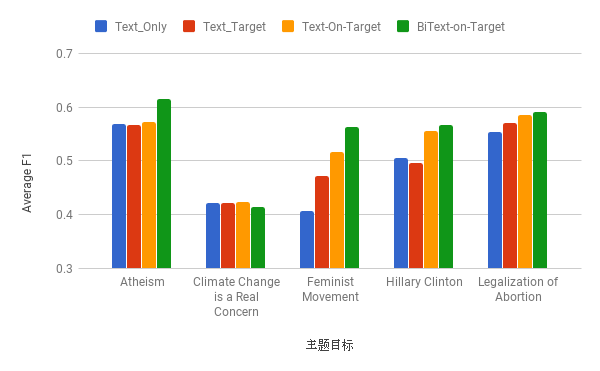
\includegraphics[width = 1.0\textwidth]{chart_seme_condi.png}
	\caption[rnn_vanish]{模型各主题目标性能分析}
	\label{semeval_model_char}
\end{figure}


对比实验各个模型在两个数据集分别调整超参数,在个模型中做多组的实验取其最优结果当做模型的预测结果。为说明各个模型在具体各个主题目标的性能,以下以英文SemEval数据集为例,计算各模型在不同主题目标下的性能,各模型在英文数据集各主题目标下性能如图~\ref{semeval_model_char}~所示,除了在”Climate Change is a Real Concern“主题目标下各模型的性能差距相对较少,具体原因由此主题目标信息的原始信息分布有关,上文已经做过相应的说明,这里就不在赘述。而其他主题目标下模型的性能还是有比较明显的差距的。

从图~\ref{semeval_model_char}~可知只用文本信息的Text-Only模型在所以主题目标的效果都不是很好,只有在”Hillary Clinton“主题目标上能稍微领先结合主题目标信息的Text-Target模型。Text-Target模型在所有主题上比Text-Only模型无明显的提升,在”Hillary Clinton“主题目标上的指标还低于Text-Only模型,这样侧面说明两个独立的LSTM模型编码主题目标信息和文本信息的模型比单独编码文本信息模型无显著的提高,独立的编码模型无法发现主题目标和文本信息相互之间作用的模式。

利用条件编码的Text-On-Target模型在各主题目标的性能相对与Text-Only和Text-Target模型都有都有显著的提升,这证明了条件编码模型能较好的结合主题目标信息和文本信息从而能找到立场分析的模式,其中的理论依据在于编码文本信息的LSTM模型是以编码主题目标信息LSTM为条件,信息从编码主题目标LSTM模型流入至编码文本信息的LSTM,在未编码文本信息前就有相应的”先验知识“,对文本信息编码的LSTM模型根据主题目标的”先验知识“,能更好抓取文本中有关立场分析的模式信息。

结合社交媒体立场分析中主题目标的信息有限和文本信息较为丰富的特点,将条件编码中对文本的编码转换成双向的LSTM模型,已达到更好编码文本信息的目的。在Semeval英文数据集上也论证了这一想法。基于上述出发点改进过后的Bi-Text-On-Target模型在除”Climate Change is a Real Concern“立场以外的其他所以主题目标的性能都优于其他三个模型。


汇总各个主题的指标,各模型的总体”支持“与“反对”立场的F1值与Micro-F1值如表~\ref{semeval_all_model}~所示。
\begin{table}[htbp]
	\caption[table123]{模型整体性能对比(SemEval数据集)}
	\label{semeval_all_model}
	\vspace{0.5em}\centering\wuhao
	\begin{tabular}{cccccccc}
		\toprule[1.5pt]
		模型& $P_{favor}$&$R_{favor}$&$F_{favor}$&$P_{against}$&$R_{against}$&$F_{against}$&$F_{average}$ \\
		\midrule[1pt]
		Text-Only&0.5364&0.5822&0.5593&0.7258&0.7329&0.7293&0.6443\\
		Text-Target&0.4564&0.6711&0.5637&0.7594&0.6224&0.6909&0.6273\\
		Text-on-Target&0.5776&0.6118&0.5947&0.7234&0.7608&0.7421&0.6684\\
		BiText-on-Target&0.5743&0.6480&0.6112&0.7396&0.7231&0.7314&0.6713\\
		\bottomrule[1.5pt]
	\end{tabular}
\end{table}

\begin{table}[htbp]
	\caption[table123]{模型整体性能对比(NLPCC数据集)}
	\label{semeval_all_model}
	\vspace{0.5em}\centering\wuhao
	\begin{tabular}{cccccccc}
		\toprule[1.5pt]
		模型& $P_{favor}$&$R_{favor}$&$F_{favor}$&$P_{against}$&$R_{against}$&$F_{against}$&$F_{average}$ \\
		\midrule[1pt]
		Text-Only&0.6465&0.6635&0.6550&0.7275&0.6769&0.7022&0.6786\\
		Text-Target&0.6297&0.6778&0.6538&0.7333&0.6299&0.6816&0.6677\\
		Text-on-Target&0.6504&0.7017&0.6761&0.7450&0.6871&0.7161&0.6961\\
		BiText-on-Target&0.6721&0.6850&0.6785&0.7146&0.7219&0.7182&0.6984\\
		\bottomrule[1.5pt]
	\end{tabular}
\end{table}

其中两个数据集中Text-Only模型取得0.644和0.678的微平均F1值,而Text-Target模型虽然在各个主题目标下的F1值接近Text-Only的值F1值,但是在总体上的微平均值只有0.627和0.667,分别少了Text-Only模型1个多点,也在一定程度上说明如果主题目标信息引入的方法不对(直接拼接向量)后,有可能导致模型的实际泛化能力还下降了,导致整体的效果还不如只考虑文本信息本身,因此在文本立场分析任务中,以合适的方式引入主题目标建立合适的模型是重要的一个环节。

以条件编码结合主题目标和文本的模型在两个数据集上都取得较好的结果,其中Text-On-Target模型在中英数据集上取得0.668和0.698的平均F1值,比Text-Only模型在两个模型中分别高了0.024和0.020,说明引入主题目标作为对文本编码的”先验知识“能显著的提高模型在文本立场分析的性能。Text-on-Target比Text-Target模型在两个数据集上高0.044和0.031的微F1值,此处提升的比对比Text-Only模型还高,说明以条件编码结合主题目标信息比直接单独拼接特征向量的方法更能挖掘文本和主题目标之间的立场关系。

对比Text-On-Target模型和BiText-On-Target模型在各数据集上的表现, BiText-On-Target在英文数据集上取得0.6712的微平均F1值,Text-On-Target模型取得了0.668的的F1值。BiText-On-Target在英文数据集上比Text-On-Target高出0.003的微平均F1值,因此在英文数据上双向LSTM模型编码文本信息比单向LSTM模型更好,这点由于双向LSTM有更好的提取文体特征的能力。但在中文数据集合上,Bi-Text-On-Target比Text-On-Target模型高出0.002。双向的LSTM模型不管对中文还是英文的文本的建模能力更强。基于主题目标信息条件双向的LSTM编码模型在四个模型中的性能最高。

上述实验论证以合适的方式引入主题目标信息可以提升文本立场分析的性能,为了验证提出的条件编码LSTM模型的有效性和不足,以下通过实验结果对比其他研究人员在文本研究中模型。由于两个数据集来源于不同的评测任务,因此分别从SemEval2016英文数据集和NLPCC2016中文数据集挑选出较好系统和本章提出的条件编码LSTM进行比较。

在SemEval数据集合上,引入以下模型是作为对比模型

(1)MITRE, SemEval2016 Twitter立场分析评测任务第一名,收集大量的无标注数据。通过分析筛选出多个\#话题标签,建立LSTM模型去预测文本的标签。先训练预测标签的模型,而后在预训练好的模型上做立场分析的任务上的微调,此模型基于大量无标注样本的迁移学习,需要大量无标注任务和手工筛选特别话题标签。

(2)TakeLab   SemEval2016 Twitter立场分析评测参赛模型,融合了随机森林,逻辑回归,支持向量机等多种机器学习的集成学习方法,各模型利用大量人工构造的特征。

(3)ECNU  SemEval2016 Twitter立场分析评测华东师范大学参赛模型,采用了传统语义特征、主题目标特征、相似性特征、情感字典特征、主题模型特征和词向量特征的特征工程的传统机器学习方法

(4) BiText-On-Target本章出的基于主题目标的条件的双向LSTM文本编码模型

四个模型在SemeEval2016的各主题目标下单个平均F1值如图~\ref{chart_semeval_best_model}~所示
\begin{figure}[htbp]
	\centering
	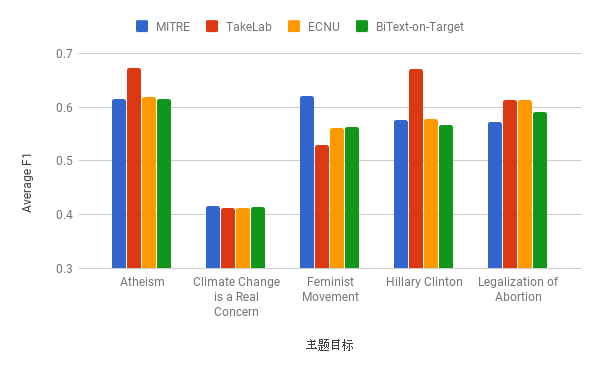
\includegraphics[width = 1.0\textwidth]{chart_semeval_best_model.png}
	\caption[rnn_vanish]{模型在SemeEval2016各主题目标平均F1值分布}
	\label{chart_semeval_best_model}
\end{figure}
所以模型在”Climate Change is a Real Concern“主题目标上的性能都较差,没有一个模型的性能超过了0.43的平均F1值。数据类标分布极度不平均,训练集与测试集分布差异大的问题的问题影响了所有模型,4个模型都没克服这个缺陷。基于特征工程的TakeLab和ECNU模型对”Legal of Abortion“主题目标的性能相对较好,基于深度学习的MITRE模型和BiText-On-Target模型相对较差,在此主题目标下,基于统计的特征具有更好的立场分析区分度。TakeLab在”Atheism“和”Hillary Clinton“主题目标的效果远高于其他模型,原因是其运用了集成随机森林,逻辑回归,支持向量机等多种分类器,模型相对强健。BiText-On-Target模型在所有的主题目标下都拥有相对稳定的效果,虽然没在任意主题目标取得最好的立场分析效果,但所有主题目标的效果都不是很差,相对于其他三个模型更加稳定和强健。

上述模型在SemEval数据集下的综合”支持“和”反对“的F1值和总体微平均F1值的性能如下表~\ref{semeval_res}~所示

评测最好的模型MITRE的的微平均F1值为0.678,本章提出的模型BiText-On-Target取得了0.671的平均F1值,此模型在评测中取得3(20)的成绩。虽然模型的性能比MITRE的相比低了0.007,但MITRE需要大量的无标注数据,TakeLab模型虽然在某些主题目标下取得较好的F1平均值,但是对于总体的”支持“和“反对”立场微平均F1值的效果不如BiText-On-Target模型。

\begin{table}[htbp]
	\caption[table123]{各模型在立场分析测试集中的性能表现(SemEval 数据集)}
	\vspace{0.5em}\centering\wuhao
	\label{semeval_res}
	\begin{tabular}{cccccccc}
		\toprule[1.5pt]
		主题目标& $F_{favor}$&$F_{against}$&$F_{average}$ \\
		\midrule[1pt]
		MITRE&0.5932&0.7633&0.6782\\
		TakeLab&0.6093&0.7273&0.6683\\
		ECNU&0.6055&0.7054&0.6555\\
		BiText-On-Target&0.6112&0.7314&0.6713\\
		\bottomrule[1.5pt]
	\end{tabular}
\end{table}

上述统计说明模型在SemEval英文数据的性能,以下将在NLPCC2016中文数据集对比评测中的模型,对比的模型如下所示

(1)RUC-MMC NLPCC2016 立场分析评测任务第一名,提取同义词,TF-IDF,n-gram等作为特征结合支持向量机和随机森林分类器。

(2)Top-Team NLPCC2016立场分析评测任务参赛模型,为每个主题目标抽取分类关键词字典。

(3) BiText-On-Target 本章提出的基于主题目标的条件的双向LSTM文本编码模型。

三个模型在SemeEval2016的各主题目标下单个平均F1值如图~\ref{chart_nlpcc_best_model}~所示
\begin{figure}[htbp]
	\centering
	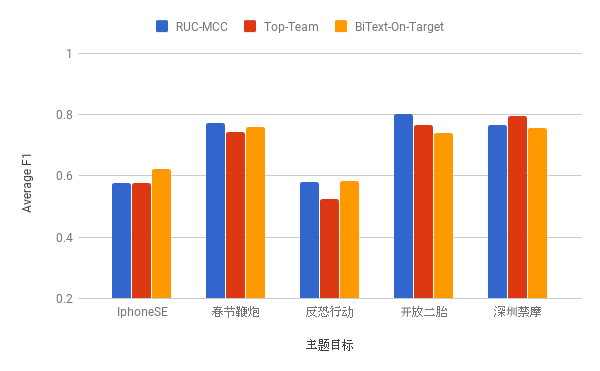
\includegraphics[width = 1.0\textwidth]{chart_nlpcc_best_model.png}
	\caption[rnn_vanish]{模型在NLPCC2016各主题目标平均F1值分布}
	\label{chart_nlpcc_best_model}
\end{figure}

本章节提出的BiText-On-Target模型在”春节放鞭炮“主题目标下取得了最好的0.75的平均F1值,RUC-MCC模型春节放鞭炮以外在其他主题模型上均有不错的性能,基于提取每个主题目标的关键字典的Top-Team在”深圳禁摩限电“主题目标上取得最好的0.794平均F1值。三个模型都有自己擅长的分析的主题目标,没有哪个模型能在所有主题目标中取得最好的指标。

上述模型在NLPCC数据集下的综合”支持“和”反对“的F1值和总体微平均F1值的性能如下表~\ref{nlpcc_res}~所示
\begin{table}[htbp]
	\caption[table123]{各模型在立场分析测试集中的性能表现(NLPCC 数据集)}
	\label{nlpcc_res}
	\vspace{0.5em}\centering\wuhao
	\begin{tabular}{cccccccc}
		\toprule[1.5pt]
		主题目标& $F_{favor}$&$F_{against}$&$F_{average}$ \\
		\midrule[1pt]
		RUC-MMC&0.6969&0.7243&0.7106\\
		Top-Team&0.6601&0.7186&0.6894\\
		BiText-On-Target&0.6761&0.7158&0.6984\\
		\bottomrule[1.5pt]
	\end{tabular}
\end{table}

本章提出的BiText-On-Target模型的性能可在NLPCC2016数据集上取得总微平均F1性能第二名,表明本章提出的BiText-On-Target模型是有效的,但是其性能和基于特征工程的RUC-MMC还有少了0.012差距,因此模型在立场分析建模上还有些许的不足,后续也可在此模型的基础上,更深入研究文本立场分析的问题。



\BiSection{本章小结}{}
本章介绍了基于条件编码LSTM模型的文本立场分析上的工作,受条件编码在文本蕴含任务上性能突破,将条件编码模型引入到文本立场分析任务。本章也简介了下SemEval2016和NLPCC2016两个社交媒体数据集,且说明评测的指标。对于立场分析中主题目标信息是否能促进文本立场分析的性能进行了探究,在两个数据集上设计了多组对比实验,实验证明以独立编码融合主题目标信息和文本信息的模型和直接单独编码文本信息的模型性能差距不大,而以条件编码融合主题目标信息和文本信息能提高文本立场分析的性能,得出以合适的方式引入主题目标信息对文本立场分析有促进作用,结合文本立场分析的特点,改进了条件编码模型,在两个数据集上的性能都优于原有模型,最好在中英文数据集上取得微平均F1值分别为0.698和0.671。通过对比两个数据集其他模型,条件编码LSTM模型均有不错的效果,表明本章提出的模型的有效性。

